\documentclass{article}
\usepackage{amsmath}
\usepackage{graphicx}
\usepackage{siunitx}
\usepackage{float}
\usepackage{gensymb}
\usepackage[dvipsnames]{xcolor}
\usepackage{sectsty}

%\setlength{\parskip}{1em}

\definecolor{color:background}{RGB}{40,40,40}
\definecolor{color:text}{RGB}{230,230,230}

\pagecolor{color:background}
\color{color:text}
\allsectionsfont{\normalfont\sffamily\bfseries}

\title{MTRL 280 Material Selection}
\author{Kelvin Hsu}


\begin{document}
    \sffamily
   	\maketitle
    \newpage

    \section*{The Design Process}
    \subsection*{What is design?}
    Design is the process of translating a new idea or a market need into the 
    detailed information from which a product can
    be manufactured.

    \subsection*{The Need Statement}
    Any design process starts with a need statement. A need statement must be solution neutral which 
    means it should not convey how a problem can be solved. "A device is required to perform the following set of design requirement" would be 
    an example of a need statement.

    \subsection*{Types Of Design}
        \begin{itemize}
            \item Original Design: A new idea or a new working principle
            \item Adaptive Design: Redesign of existing product that seeks improvement in performance
            \item Variant Design: Change of dimension or detailing without a change of 
            function or method of achieving it.
        \end{itemize}


    \section*{Material Information}

    \subsection*{Structural Property}
        Structural properties are properties that changes with the dimension, geometry, and shape of an object. Design is usually specified with structural properties.
        \begin{itemize}
            \item Force at Failure($N$): How much force is required to break the object under force.
            \item Stiffness($N/m$): How much deformation there is when a force is applied. This is a structural property
                                    because it depends on the geometry and size of the object. Ex. Increasing 
                                    the thickness of an object also increase its stiffness.
            \item Electrical Resistance($\ohm$)
        \end{itemize}

    \subsection*{Material Property}
        Material Properties are properties that does not change with the dimension, geometry, and shape of an object.
        It has been normalized.
        \begin{itemize}
            \item Failure Stress ($N/m^{2}$): Stress at failure
            \item Elastic Modulus ($N/m^{2}$): measures how much a subject deforms when a stress is applied to it.
            \item Resistivity ($\ohm m$)
            \item Strength($\sigma_{f}$)
        \end{itemize}

    *There is usually a complementary material property for a structural property.

    \paragraph*{Strength\newline}
    Strength is defined differently for different material.
    \begin{itemize}
        \item Metal: The stress at which the stress-strain curve for axial loading deviates by 0.2$\%$
                     from the linear elastic line. (find 0.2$\%$ on strain axis then draw a line parallel to Young's Modulus, the intersection between the drawn line and the actual curve is the strength)
        \item Polymer: The stress at which the stress-strain curve becomes non-linear.
        \item Ceramics and Glasses: Depends on the mode of loading, for tension - fracture strength($\sigma_{t}$), for compression - 
                                    crushing strength ($\sigma_{c}$). Strength can also be measured in bending - flexure strength or modulus of rupture.
    \end{itemize}


    \paragraph*{Toughness\newline}
    Area under the stress-strain curve, the amount of energy required to fracture or the amount
    of energy stored while the material plastically deform.

    \paragraph*{Fracture Toughness\newline}
    How resistant(amount stress) a material is to propagation of an existing crack.

    \noindent *Ceramics have low fracture toughness(cracks in concrete) and low toughness(easy to fracture); polymers have high toughness(not easy to fracture) and low fracture toughness
    (easy to break once there is a crack in it), think of tapes.

    \paragraph*{Thermal Conductivity\newline}
    The rate at which heat is conducted through a material when temperatures are fixed. It is a measure of whether heat transfers quickly(high) or slowly(low).
    \paragraph*{Thermal Diffusivity\newline}
    It is the rate of an object with non uniform temperature reaches thermal equilibrium. It is a measure of whether the object 
    heats up fast(high) or slowly(low).

    \subsection*{Mechanical Loading}
    \begin{itemize}
        \item Tie - in tension
        \item Beam - in bending
        \item Shaft - in torsion
        \item Column - in compression
    \end{itemize}

    \section*{Material Property Chart}
    A graph containing 2 material properties on the two axes.

    \section*{Material Selection Steps}
    The first step in material selection is to define the function, objective, constraint, and free variables 
    from the design requirement.
    
    \begin{itemize}
        \item Function: what the component must be able to do
        \item Objective: a parameter to optimize (maximize or minimize)
        \item Constraint: the condition the design must meet (hard or soft)
        \item Free Variable: what can be changed by the designer (material is always a free variable)
    \end{itemize}

    The second step in material selection is to screen and rank the materials that can be used for the design.

    \subsection*{Screening}
    \begin{itemize}
        \item Engineering Design must be unbiased, therefore all materials are equally possible initially.
        \item Constraints can be used to screen material.
    \end{itemize}

    \subsection*{Ranking}
        Ranking is to rank the remaining materials after screening base on their performance.
        Constraints and objectives are usually coupled through a free variable. The Constraints
        are used to eliminate the free variable in the objective equation. The resulting parameter 
        to be maximized(optimized) is a material property that is refer to as the materials index. The 
        objective equation can usually be separated into a functional, a geometry, and a material part.
        Always isolate for free variable in the constraint equation and substitute into the objective equation.


    \section*{Shape Factor ($\phi$)}
    Measure of improvement in performance by changing shape. It is the ratio between the stiffness
    of a given shape and a reference shape. Shape factor does not depend on size. The higher the shape
    factor, the better the shape performs compare to the reference shape. The reference shape is often a 
    solid square.

    \subsection*{Shape Factor in Bending}
    \begin{align*}
        &S = \frac{EI}{L^{3}}\\
        &I_{ref} = \frac{A^{2}}{12}\\
        &\phi^{Elastic}_{Bending} = \frac{S}{S_{ref}} = \frac{I}{I_{ref}} = 12\frac{I}{A^{2}}
    \end{align*}

    \subsection*{Limits To Shape Factors}
    \begin{enumerate}
        \item Empirical Limits
            \begin{itemize}
                \item Imposed by manufacturing Constraints
                \item Difficulty or expensive to make a given shape
                \item Limitations may be intrinsic to material
            \end{itemize}
        \item Competing Failure Mechanism
            \begin{itemize}
                \item New mode of failure may be more dominant
                \item Reduce wall thickness lead to buckling...
            \end{itemize}
    \end{enumerate}

    \section*{Hybrid Material}
    Hybrid material is designed to fill the holes on the material property chart.
    It is a combination of two or more materials in a predetermined 
    configuration, relative volume, and scale, optimally serving a specific 
    purpose.

    \subsection*{Types of Hybrid Material}
        \begin{enumerate}
            \item Composite - made up of 2 materials, one for matrix and the other for reinforcement.
            \item Sandwich - made up of 2 materials, one is the core, one is the outer surface.
            \item Lattice - similar to form, but with a highly tailored order of material. 
            \item Segment - comprised of structural units of material that can be combined in either 2D or 3D.
        \end{enumerate}
    
    \subsection*{Property of a Hybrid Material}
    There are 4 average behavior a hybrid material can have depending on how the hybrid material
    is designed.
        \begin{enumerate}
            \item Greatest Of Both - hybrid with the best properties of both components
            \item Rule Of Mixture - weighted average of the properties of the two material base on their volume fraction
            \item Harmonic Means - when the property is more dominated by the weaker one of the components
            \item Least Of Both - hybrid with the weakest properties from one of the components
        \end{enumerate}

    \paragraph*{Density\newline}
    Density of a hybrid material obeys the rule of mixture such that it solely depends on the volume fraction
    of the components.
    \begin{equation*}
        \rho = V_{f1}\rho_{1} + V_{f2}\rho{2}
    \end{equation*}

    \paragraph*{Elastic Modulus\newline}
    Elastic Modulus of a hybrid material not only depends on the volume fraction, but also the 
    configuration(orientation, direction...) of the hybrid material. In this case, to predict 
    the hybrid material's property, a lower bound and a higher bound of the elastic modulus are found
    instead of calculation every single combinations.
    \vspace{1em}

    \noindent The upper bound estimate is given by when 2 materials are 2 fibers oriented parallel to the direction of loading.
    where the deformation of the first component is equal to the deformation of the second.

    \begin{equation*}
        \epsilon_{hybrid} = \epsilon_{1} = \epsilon_{2} 
    \end{equation*}

    \noindent The stress for the hybrid material is therefore,
    \begin{equation*}
        \sigma_{hybrid} = \sigma_{1}V_{f1} + \sigma_{2}V_{f2}
    \end{equation*}

    \noindent The upper bound estimate of the elastic modulus is then,
    \begin{equation*}
        E = \frac{\sigma}{\epsilon}= V_{1}E_{1} + V_{2}E_{2}
    \end{equation*}


    \noindent The lower bound estimate is given by when 2 materials are 2 fibers are oriented perpendicular to the direction of loading.
    The stress in the two materials must be the same.

    \begin{equation*}
        \sigma_{hybrid} = \sigma_{1} = \sigma_{2}
    \end{equation*}

    \noindent The strain parallel to the loading direction must only sum to give the imposed strain.
    \begin{equation*}
        \epsilon_{hybrid} = V_{f1}\epsilon_{1} + V_{f2}\epsilon_{2}
    \end{equation*}

    \noindent The lower bound estimate of the elastic modulus is then,
    \begin{equation*}
        \frac{1}{E} = \frac{V_{f1}}{E_{1}} + \frac{V_{f2}}{E_{2}}
    \end{equation*}

    \subsection*{Sandwich Panel}
    Sandwich panel can be used as a light stiff panels in bending. Since most materials that
    has a low density also has a low elastic modulus. To achieve both objectives, notice that
    for a body in bending, most of the load is carried by the surface material $=>$ high modulus material for the surface, low
    density material for the core.
    \vspace{1em}

    \noindent The modulus of a sandwich panel depends on the overall bending and from shear of the core, it is also 
    sensitive to the volume fraction of the components.

    \paragraph*{Types Of Failure For A Sandwich Panel}
    \begin{enumerate}
        \item Core Shear
        \item Face Yield
        \item Face Buckling
    \end{enumerate}

    \subsection*{Potential of Lattice Structure}
    Stretch Dominated Lattices  - perform better than foam because of highly order cell wall. 

    \section*{Multiple Constraints}
    When there are 2 constraints(two material indices), which constraint dominates?
    Find the constraint that is more limiting such that when that constraint is met, the 
    other constraint is also met.
    
    \subsection*{Strategy}

        \begin{enumerate}
            \item Make a preliminary short list of materials by consecutive application of materials indices 
                  and material property charts.
            \item From the initial list, make a table and calculate the free variable, objective
            \item For each material, look at the prediction of the free variable/objective and pick the one 
                  that is most limiting.
            \item From the table, pick the best material.
        \end{enumerate}

    However, we cannot be sure that the initial screening did not screen out good potential material.
    Computer software is used to graph all material's variables with respect to different constraints and compare 
    which material is best.
    
        \section*{Compound Objectives}
        When they are competing objectives, one must look for trade offs. 
        In Figure \ref{fig:trade_off_graph}, a "trade off surface" is defined, which is a short list of 
        possible, optimal solutions(Pareto Set). Alternatively, one of the objective can be turned into the constraint where 
        the maximum value for an objective is fixed.

        \begin{figure}[H]
            \centering
            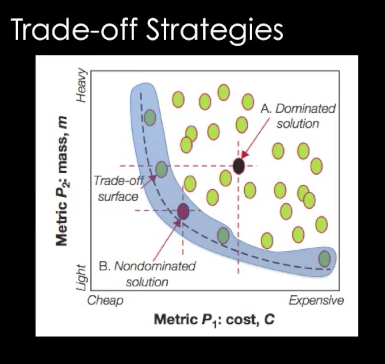
\includegraphics[width=10cm]{figures/trade_off_graph.PNG}
            \caption{Cascode Amplifier}
            \label{fig:trade_off_graph}
        \end{figure}
        
        \section*{Penalty Function}
        Using tradeoff surfaces helps us to narrow down to a set of good possible 
        solutions; however, there is no way to quantitively compare how good the different 
        solutions are within the Pareto set. A penalty function compares different options from the 
        Pareto set.\par

        A penalty function is a linear combination of all objectives.

        \begin{equation*}
            Z = \alpha_{1} P_{1} + \alpha_{2} P_{2}+...
        \end{equation*}

        where alpha is a exchange constant that measures the rate of change of the 
        penalty function with respect to each objective.

        \begin{equation*}
            \alpha_{i} = \frac{\delta Z}{\delta P_{i}}
        \end{equation*}

        \subsection*{Example}
        Let Z be a penalty function for mass and cost.
            \begin{align*}
                Z = C + \alpha m\\
                m = -\frac{C}{\alpha} + \frac{Z}{\alpha}
            \end{align*}
        Different Z can be plotted on the graph of 2 objectives, and the best option will lie in the 
        bottom left corner where Z is at a minimum.

        \subsection*{Exchange Constant}
        Obtaining the exchange function is difficult. It can be found based on engineering criterial or 
        market research, or political or socio-economic policy. The exchange function does not have to be a constant.

        \section*{Process Selection}
        \begin{itemize}
           \item Function: What must the process do?
           \item Constraints: What technical limits must be met?
           \item Objective: What is to be maximized or minimized?
           \item Free Variable: Choice of process and process-operating conditions. 
        \end{itemize}

        \subsection*{Screening}
        \subsubsection*{Important Processing Attribute}
        \begin{itemize}
            \item Material Compatibility: what process can be used for that specific material?
            \item Size and Shape
            \item Tolerance and surface roughness
        \end{itemize}
        Chart can be used to perform screening on processes.
        
        \subsection*{Ranking Potential Processes}
        How to keep the cost down?
        \begin{enumerate}
            \item Keep it standard(buy, don't make) 
            \item Keep it simple
            \item Do not over specify
        \end{enumerate}

        \subsection*{Process Cost Model}
        Process is the sum of the costs of the resources it consumes

        \begin{equation*}
            C = [mC_{m}] + \frac{C_{t}}{n} + \frac{\dot{C_{L}}}{\dot{n}}
        \end{equation*}

        \begin{equation*}
            \frac{\text{Cost}}{\text{Component}} = \frac{\text{Material + tooling + overhead + power + space + $\dots$ }}{\text{Component}}
        \end{equation*}
        *Normalized to cost per part.

        \begin{itemize}
            \item material cost (constant)
            \item tooling cost (depends on batch size)
            \item overhead cost (operating cost, power, water...)(constant)
        \end{itemize}

       \section*{Material Selection and Environment} 
       \subsection*{Life Cycle Analysis}
       \begin{itemize}
           \item Material Production
           \item Product manufacturing
           \item Transport
           \item Product used
           \item Product Disposal
       \end{itemize}

       \subsection*{Eco-Attributes of a Material}
       Embodied Energy: the fossil-fuel energy consumed in making 1 kg of  material.
       CO2 Footprint: the amount of CO2 produced in the production of 1 kg of material.

       \begin{equation*}
            E = m * H_{p} = AL \rho H_{p}
       \end{equation*}
       where $H_{p}$ is the embodied energy(j/kg)





        
        

\end{document}